\documentclass[sigconf]{acmart}

\usepackage{dirtytalk}
\graphicspath{ {images/} }

\usepackage{graphicx}
\usepackage{hyperref}
\usepackage{todonotes}

\usepackage{endfloat}
\renewcommand{\efloatseparator}{\mbox{}} % no new page between figures

\usepackage{booktabs} % For formal tables

\settopmatter{printacmref=false} % Removes citation information below abstract
\renewcommand\footnotetextcopyrightpermission[1]{} % removes footnote with conference information in first column
\pagestyle{plain} % removes running headers

\newcommand{\TODO}[1]{\todo[inline]{#1}}

\begin{document}
\title{Big Data Analytics in Higher Education Marketing}


\author{Ashley Miller}
\orcid{HID329}
\affiliation{%
  \institution{Indiana University}
  \date{October 2017}
}
\email{admille@iu.edu}



% The default list of authors is too long for headers}
\renewcommand{\shortauthors}{B. Trovato et al.}


\begin{abstract}
While the collection of vast amounts of data in the world of higher education has occurred for decades, the use of big data applications and analytics is fairly new to this environment. There is a need to understand how the use of big data analytics can help institutions determine student behavior as well as stay relevant in a digital and evolving age of technological advances, tools, and skills. The higher education space is changing as the population of students going to college is on the decline which increases competition and the need for institutions to be more strategic in their efforts for attracting students to their institutions. We will explore at a very high level how higher education could utilize big data analytics to inform marketing initiatives in recruiting and enrolling students as well as what potential challenges and considerations could impact this process. 
\end{abstract}

\keywords{i523, hid329, big data, higher education, marketing, analytics, data-driven decision making}


\maketitle

\section{Introduction}

Today's colleges and universities are drowning in data \cite{Daniel2015}. With the emergence of big data, institutions are now faced with providing useful analysis and reports to a variety of stakeholders including administrators, professors, as well as to the students themselves \cite{Daniel2015}. A variety of challenges lie in the path of institutions using big data effectively such as finding the necessary skill set for staff, technology tools and resources, as well as understanding then what to do with the data collected to better inform decision making. 
While there is literature that addresses utilizing big data for learning analytics and even course enrollment and development, as Daniel states, there is still \say{limited research into big data in higher education} \cite{Daniel2015}. Higher education could benefit from using big data analytics in their marketing efforts for recruiting and enrolling students as well as identifying what gaps may still exist in the quest to understand today's college student in their college search process. 


\section{Current Environment}

According to the \textit{Western Interstate Commission for Higher Education (WICHE)}, the projected number of high school graduates will decline over the course of the next decade \cite{Bransberger2017}. Meanwhile, the number of four-year institutions in the United States has increased with more than 3,000 available college options \cite{EducationStatistics2015}. Increased competition and fewer students have made the higher education marketplace crowded and convoluted. There are a variety of factors that go into a student's decision on where to attend and ultimately what area to study. In their 2013 trends report, the Lawlor group  identified a number of aspects that will impact the higher education landscape, among those included are \cite{Research2014}:

\begin{itemize}
\item The demographics of today's college student is changing with more women attending college than men in addition to an increase in ethnic and socio-economic diversity as well as first-generation students \cite{Bransberger2017}.

\item The college search process today happens primarily in the digital space which includes third-party websites, email, social media, and digital advertising \cite{Geyer2016}. This \textit{Generation Z} grew up in a technology rich and connected environment which means that colleges have to also be constantly on in this space to effectively recruit and enroll students \cite{Geyer2016}.

\item The need to showcase the \textit{value} of going to college, not only through the quality of education received relative to the price paid but also through outcomes-level data, including retention and placement rates and even starting salaries of recent graduates. 
\end{itemize}

With these trends in mind, there is a need for institutions to be more targeted in their marketing efforts. Big data analytics can be used to help assess the impact of these trends as well as how institutions can make better decisions with these techniques.

\section{Big Data Analytics to Segment by Demographics}
Big data can be one way to better inform these efforts and also help with the return-on-investment (ROI) for advertising and marketing related efforts. Other universities have capitalized on utilizing big data in attracting students. For instance, St. Louis University described a process of retroactively looking at demographics of students who succeeded at the university and had high satisfaction scores \cite{Selingo2017}. This information coupled with nearly 100 other data points gave insight to the admissions team when exploring new markets as well as identified clusters of students that may be interested in attending St. Louis University \cite{Selingo2017}. The university was then able to develop a targeted digital campaign in these areas that they believed included students who would be a good fit for the university. With the reliance on big data, St. Louis University was able to reduce costs as the need to mass market went away and ultimately increased enrollment and retention rates \cite{Selingo2017}.  

\section{Big Data Analytics to Understand Behavior Online}
The web environment is common tool in college exploration as a report by Ruffalo Noel Levitz shows that three out of four high school students utilize an institution's website as their most used resource when exploring colleges \cite{Geyer2016}. Web analytics provides a wealth of information on users such as how much time is spent on certain pages, bounce rate, paths in website exploration and ultimately conversion rates when various goals are completed such as scheduling a tour or filling out an application for college \cite{Omidvar2011}. Google Analytics is one tool used to track and evaluate efforts on websites. Higher education institutions could take advantage of this tool by tracking top pages viewed, geography and age of visitors, as well as areas where they may be losing students in the information search process. With this data, institutions can identify opportunities for improvement in ensuring students are finding the information they need in a timely and efficient way as well as develop customized marketing efforts to invite students back into the experience to complete various calls-to-action. 

\section{Big Data Analytics to Convey Value}
Utilizing big data to understand outcomes of current students, and ultimately graduates, can help tell the value story to prospective students \cite{Research2014}. By tracking the experiences among current students during their four (or more) year college career, predictive analytics could be implemented to determine which combination set of experiences best contribute to the success of a student. Temple University utilized predictive analytics to increase graduation rates by sending messages to students who were considered to be ``at risk for dropping out'' based on financial aid data \cite{Zinshteyn2016}. This similar type of approach could be utilized in marketing efforts as well. If a profile of student could be created based on existing data and therefore create an ability to predict the future actions of prospective students, then marketing messages could be more tailored based on where that prospective student is in the enrollment funnel. 

\section{Challenges}
In order for the use of big data analytics in higher education marketing to be successful, there are basic measures that have to be met. Marsh et. al outlines some key considerations when using big data analytics for effective decision making which include: accessibility, quality, timeliness, and motivation to use \cite{Marsh2006}. These same factors can be also impact the use of big data analytics in a higher education setting. 

\subsection{Accessibility}
Typically, institutional research offices have been the primary house for student data collected over time but that doesn't mean it's the only place where data lives \cite{Picciano2012}. As Daniel state, there is also data in higher education that lives across a number of areas in a wide variety of formats \cite{Daniel2015}. With this, accessing data can be a challenge as there is no central system or warehouse. Depending on the type of data needed, the sources can be siloed which means that the data sources are not connected to one another to provide a complete picture. Further, the level of permissions to access data can also vary which can make it difficult for marketers to access. 

\subsection{Quality}
Coupled with the fact that data across an institution can live in multiple places, there are issues around the quality of data \cite{Daniel2015}. The disparity of data sources can lead to quality concerns but also the skill set of those who maintain or utilize the data. If no standard processes exist for data cleaning, integration, reporting, or interpretation, then the risk of having invalid conclusions increases \cite{Marsh2006}. Decisions made on inaccurate data could potentially be costly for institutions. 

\subsection{Timeliness}
There can be issues with timeliness in a variety of ways. Alignment on the objectives for data analysis can require input from multiple stakeholders which takes time. The aspects involved in processing the data itself could involve a significant amount of time, people, and resources. Often times, decision making for marketing purposes needs to happen quickly and there can be a gap between obtaining the needed information and when decisions need to be made \cite{Marsh2006}. 

\subsection{Motivation}
There is also a underlying cultural aspect to using big data analytics in the right way across an institution. With the silos that exist in higher education, collaborating across departments and sharing information overall can help to forge better working relationships. Successful efforts rely on the involvement of multiple departments including information technology (IT) \cite{Daniel2015}. The importance and message about utilizing big data analytics has to come from leadership for others to be equally motivated. 

\section{Possible Solutions}

While significant challenges can exist in utilizing big data analytics to inform marketing initiatives in higher education, there are possible solutions to explore. One way to overcome the challenge of accessibility would be to create a central area where data could live. This would also allow the opportunity for others to access data and create consistency across the institution. Having a central system would also help with the data quality aspect if the the format of the data was consistent in the way it was stored, presented, and accessed. Along with creating a central area, a standardized data flow would also be beneficial. In Figure \ref{fig:figure1}, Eduventures outlines a proposed data flow within the area of higher education \cite{Wiley2016}. 

\begin{figure}[p!]
    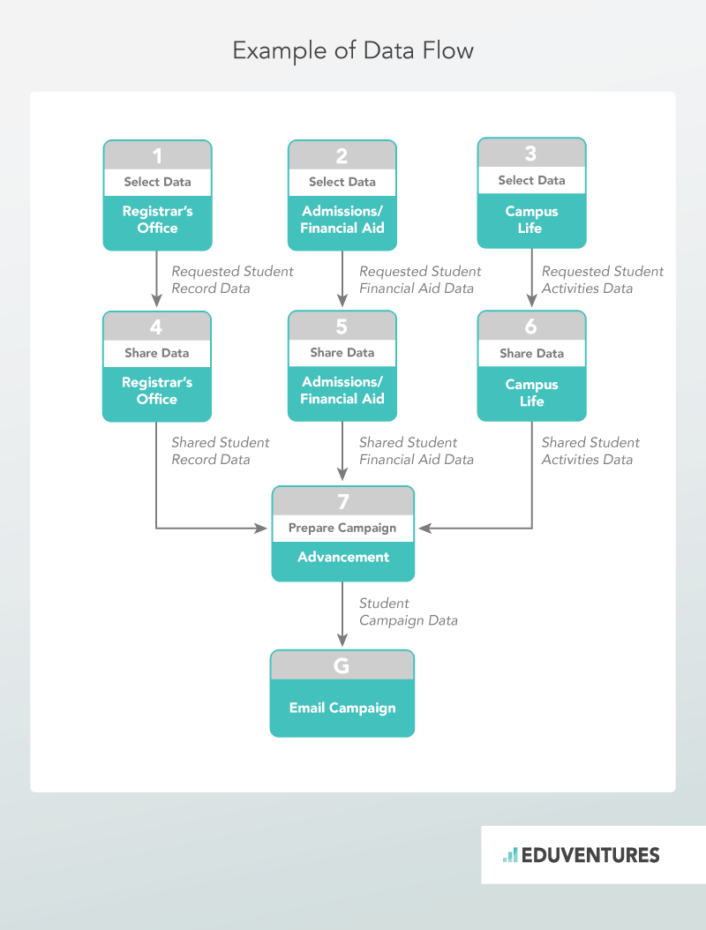
\includegraphics[width=0.5\textwidth]{dataflow2}
    \caption{Example of a data flow \cite{Wiley2016}}
    \label{fig:figure1}
\end{figure}

\section{Other Considerations}
Throughout this process of exploring the use of big data analytics for higher education marketing, there are other factors to consider. With the collection, analysis, and use of big data, what implications does this pose to data security and privacy issues among students? As stated by Slade and Prinsloo, ethical issues can come into play regarding data ownership and governance \cite{Slade2013}. Given that higher education institutions are faced with an increased level of scrutiny, what protocols have to be put into place to ensure the safety of students' data? Further, what level of accountability is assigned with the different areas/persons that are in need of the data to inform decision making? There are also policy issues to consider regarding what kind of data can be collected on students and how and where this information should be stored. 

\section{Conclusions}

Competition for today's student will only increase with changing educational needs and offerings, including development of emerging degree programs as well as delivery. For marketers in higher education, they need to have access to necessary data about current as well as prospective students to better tailor messaging and marketing efforts appropriately. With this, the validity of available data is key as making decisions based on incomplete data can be problematic and costly for an institution. Given the nature of the web environment that is constantly changing, obtaining data in a timely manner is crucial so action can be taken at the right time. Insights around data are only as good as the people that make use of them so creating a culture within an institution that motivates others to make data-driven decisions is imperative for these efforts to be successful.   

\section{Acknowledgements}

The author would like to thank Gregor von Laszewski at Indiana University Bloomington for his instruction and feedback as well as Juliette Zerick for providing a first review and recommendations for improvement. 




\bibliographystyle{ACM-Reference-Format}
\bibliography{report} 




\end{document}
